% XTAL: eXplainable Tail-latency Adaptive controLler
% ACM SIGOPS / IEEE format — 12 pages
% Target: Middleware 2026 / SoCC 2026

\documentclass[sigconf,natbib=false]{acmart}

% ── Packages ──────────────────────────────────────────────────────────────────
\usepackage{booktabs}
\usepackage{graphicx}
\usepackage{listings}
\usepackage{microtype}
\usepackage{xspace}
\usepackage{amsmath}
\usepackage{algorithm}
\usepackage{algorithmic}
\usepackage{subcaption}
\usepackage{hyperref}

% ── Macros ────────────────────────────────────────────────────────────────────
\newcommand{\xtal}{\textsc{XTAL}\xspace}
\newcommand{\pnn}[1]{p$_{#1}$}
\newcommand{\ms}{\,ms\xspace}

% ── Metadata ──────────────────────────────────────────────────────────────────
\title{\xtal: Explainable Closed-Loop Tail-Latency Control\\
       for Strict-Deadline Distributed Streaming Pipelines}

\author{Akanksha Garg}
\email{ag2671@rit.edu}
\affiliation{%
  \institution{Rochester Institute of Technology}
  \city{Rochester}
  \state{New York}
  \country{USA}
}

\author{Hrithik Manoj Gaikwad}
\email{hg3916@rit.edu}
\affiliation{%
  \institution{Rochester Institute of Technology}
  \city{Rochester}
  \state{New York}
  \country{USA}
}

\begin{abstract}
Strict-deadline streaming pipelines—real-time analytics, autonomous perception—
are governed by tail latency (\pnn{99}/\pnn{999}) rather than average throughput.
Existing engines such as Apache Flink and Kafka expose powerful knobs for
checkpointing, buffering, and parallelism, yet no production system closes the
loop between runtime telemetry and these knobs to actively suppress tail spikes.
We present \xtal, the first cross-layer, closed-loop tail-latency controller for
a real Kafka\,+\,Flink streaming stack.
\xtal operates a 10\,s control loop: it observes a six-dimensional system state
via Prometheus, selects one of 14 discrete configuration presets using an
XGBoost contextual bandit, applies the action through the Flink REST API and
Kafka AdminClient, and generates per-decision SHAP feature attributions that
explain \emph{why} each knob was changed.
A hard safety layer enforces correctness constraints independently of the
learned policy.
We evaluate \xtal on the NEXMark benchmark under three load patterns
(steady, 10$\times$ burst, TaskManager failure) against three baselines:
Flink defaults, the best hand-tuned static configuration, and a
threshold-based reactive autoscaler.
\xtal reduces mean \pnn{99} latency by up to \textbf{64\%} during burst events
and cuts SLA violation rate from \textbf{22\%} to \textbf{1.7\%} under failure injection,
recovering 2.3$\times$ faster than the best static baseline,
with a per-decision control overhead under 220\ms.
\end{abstract}

\keywords{tail latency, streaming systems, explainable AI, reinforcement learning,
          Apache Flink, Apache Kafka, closed-loop control}

\begin{document}

\maketitle

% ── Sections (included from separate files) ───────────────────────────────────
% ── §1  Introduction ──────────────────────────────────────────────────────────
\section{Introduction}
\label{sec:intro}

Distributed streaming pipelines increasingly support applications with
hard real-time constraints: real-time financial fraud detection, autonomous
vehicle perception stacks, and sub-second interactive analytics.
In these systems, \emph{tail latency}---the \pnn{99} or \pnn{999}
end-to-end processing delay---rather than average throughput determines
whether a deadline is met~\cite{dean2013tail}.
A single slow request that crosses a 500\ms SLA boundary is a failure
regardless of what the mean latency is.

Modern stream processing engines, Apache Flink~\cite{carbone2015flink}
and Apache Kafka~\cite{kreps2011kafka} chief among them, have rich knob
spaces: checkpoint intervals govern fault-tolerance overhead;
buffer timeouts trade batching efficiency for added latency;
operator parallelism determines how evenly load is distributed.
Yet these knobs are set \emph{statically} at deployment time.
When load spikes, a TaskManager fails, or a noisy neighbour contends for
CPU, the configuration that was optimal at startup becomes harmful.
Production operators respond with manual re-tuning or coarse autoscalers
that react too slowly and overshoot~\cite{welsh2001seda}.

We identify three structural gaps in the state of the art:
\begin{enumerate}
  \item \textbf{No cross-layer view.} Tail spikes emerge from interactions
    across the ingest layer (Kafka consumer lag), the execution layer
    (Flink buffer backpressure), and the state layer (checkpoint stalls).
    Existing autoscalers address at most one layer.
  \item \textbf{No closed-loop learning.} Rule-based threshold systems
    react but do not generalise. They require hand-crafted thresholds that
    vary by workload and cluster configuration.
  \item \textbf{No explainability.} Even if a controller works, operators
    need to understand its decisions to trust it in production.
\end{enumerate}

We present \xtal (\textbf{eX}plainable \textbf{T}ail-latency
\textbf{A}daptive contro\textbf{L}ler), a system that closes all three
gaps simultaneously.
\xtal runs a 10-second control loop that: (i)~collects a six-dimensional
telemetry snapshot from Prometheus; (ii)~selects a joint Flink+Kafka
configuration from a discrete action space using an XGBoost contextual
bandit trained online; (iii)~applies the configuration through real APIs;
and (iv)~produces per-decision SHAP feature attributions that show which
telemetry signal drove the control decision.
A hard safety layer enforces correctness invariants (e.g., checkpoint
interval $\geq 500$\ms) independently of the learned policy.

\paragraph{Contributions.}
\begin{itemize}
  \item \xtal, the first closed-loop, cross-layer, explainable
    tail-latency controller for a real Kafka\,+\,Flink stack~(\S\ref{sec:design}).
  \item A baseline characterisation study of where tail spikes originate
    under steady, burst, and failure conditions~(\S\ref{sec:motivation}).
  \item An online XGBoost contextual bandit formulation with a provably
    safe action space and SHAP explainability, requiring no offline
    training~(\S\ref{sec:design}).
  \item An evaluation on NEXMark benchmarks showing up to 38\% \pnn{99}
    reduction and 7$\times$ lower SLA violation rate versus the
    next-best baseline~(\S\ref{sec:eval}).
\end{itemize}

% ── §2  Background ────────────────────────────────────────────────────────────
\section{Background}
\label{sec:background}

\subsection{Tail Latency at Scale}
Dean and Barroso~\cite{dean2013tail} established that at scale, even a
small fraction of slow responses dominates the perceived latency of a
system: a service with 1\% of requests at 1\,s latency sees \pnn{99}
at that level regardless of the median.
This ``long tail'' effect is amplified in multi-stage pipelines because
each stage adds delay, and the slow path of each stage compounds.

\subsection{Apache Flink}
Apache Flink~\cite{carbone2015flink} is a stateful dataflow engine that
executes directed acyclic operator graphs over unbounded streams.
Key knobs relevant to tail latency:
\begin{itemize}
  \item \textbf{Checkpoint interval} ($c$): Flink snapshots operator
    state to durable storage every $c$\ms via a Chandy-Lamport barrier
    protocol. Short intervals increase fault-tolerance but add barrier
    overhead and stall operator progress.
  \item \textbf{Buffer timeout} ($b$): Flink batches output records in
    network buffers for up to $b$\ms before flushing.
    Low $b$ reduces latency; high $b$ increases throughput.
  \item \textbf{Parallelism} ($p$): the number of parallel subtasks
    per operator. Under-parallelism causes queue buildup; over-parallelism
    wastes slots and increases coordination overhead.
\end{itemize}

\subsection{Apache Kafka}
Kafka~\cite{kreps2011kafka} is the standard ingest layer for Flink
pipelines. Producer-side \texttt{linger.ms} delays sending to allow
batch accumulation; high values increase throughput but add latency to
events at the leading edge of a burst.
Consumer lag (records not yet consumed by Flink) is a leading indicator
of backpressure propagation.

\subsection{Explainable AI (XAI)}
SHAP (SHapley Additive exPlanations)~\cite{lundberg2017shap} assigns to
each feature a contribution value that satisfies the Shapley axioms
(efficiency, symmetry, dummy, additivity).
For tree-based models, \texttt{TreeExplainer} computes exact SHAP values
in $O(TLD^2)$ time, where $T$ is the number of trees, $L$ the number of
leaves, and $D$ the maximum depth---making it practical in a 10-second
control loop.

\subsection{Contextual Bandits}
A contextual bandit selects one of $K$ actions given a context vector,
observes a scalar reward, and updates a policy~\cite{sutton2018rl}.
Unlike full RL, there is no credit-assignment across time steps, which
simplifies online learning and analysis.
We use XGBoost~\cite{chen2016xgboost} as the reward predictor because:
(a)~it is natively interpretable via SHAP;
(b)~it handles tabular, non-stationary data well;
(c)~online retraining is fast ($<$\,100\ms for $<$\,10k samples).

% ── §3  Motivation ────────────────────────────────────────────────────────────
\section{Motivation: Where Does Tail Latency Come From?}
\label{sec:motivation}

To motivate \xtal, we characterise the uncontrolled Kafka\,+\,Flink
pipeline under three load patterns and four static configurations.
This study answers two questions:
(1)~Under what conditions does tail latency spike, and how quickly?
(2)~Which internal signal (\texttt{inPoolUsage} vs.\
checkpoint duration vs.\ consumer lag) spikes first?

\subsection{Experimental Setup}
We run Flink 1.18 (1 JobManager, 3 TaskManagers, 2 slots each) and
Kafka 3.6 in Docker on a single host.
The workload is NEXMark Query~5 (sliding window auction join) driven
by our load generator at 5{,}000~events/s.
Metrics are scraped via Prometheus at 5-second intervals.
We test four static configurations:
\begin{itemize}
  \item \textbf{Default:} checkpoint=5\,s, buffer\_timeout=100\ms, linger=5\ms
  \item \textbf{Low-latency:} checkpoint=500\ms, buffer\_timeout=0\ms, linger=0\ms
  \item \textbf{High-throughput:} checkpoint=10\,s, buffer\_timeout=100\ms, linger=50\ms
  \item \textbf{Hand-tuned:} checkpoint=2\,s, buffer\_timeout=10\ms, linger=5\ms
\end{itemize}

\subsection{Steady Load}
Under constant 5{,}000~events/s, all configurations achieve \pnn{99}
below the 500\ms SLA, with the default configuration exhibiting
\pnn{99}\,$\approx$\,180\ms and periodic spikes to 350\ms coinciding
with checkpoint barriers (visible as \texttt{lastCheckpointDuration}
pulses in Prometheus).

\subsection{Bursty Load}
At $t=30$\,s, throughput jumps 10$\times$ to 50{,}000~events/s for 10\,s.
The sequence of events is consistent across all configurations:
\begin{enumerate}
  \item Kafka consumer lag grows within 1\,s as Flink cannot drain the
    partition at burst rate.
  \item Input buffer usage (\texttt{inPoolUsage}) saturates to $>$0.9
    within 5\,s, triggering Flink backpressure.
  \item Checkpoint barriers stall behind full buffers;
    \texttt{lastCheckpointDuration} spikes from $\sim$850\ms to
    $>$8{,}000\ms.
  \item End-to-end \pnn{99} rises to 1{,}200--3{,}400\ms (2.4--6.8$\times$
    the SLA) and remains elevated for 25--60\,s after the burst ends.
\end{enumerate}
The \textbf{hand-tuned} configuration recovers fastest (28\,s) because its
shorter checkpoint interval (2\,s) limits barrier alignment overhead.
The \textbf{high-throughput} configuration is worst, taking 62\,s to recover.

\textbf{Finding~1:} Consumer lag and input buffer usage are leading
indicators of a tail spike; checkpoint duration spikes are the mechanism
that sustains the spike.

\subsection{Failure Injection}
We kill one TaskManager at $t=45$\,s.
Flink detects the failure and triggers job restart with a savepoint.
During recovery (30--50\,s), \pnn{99} is undefined (no results produced).
After recovery, the two remaining TaskManagers are overloaded:
consumer lag grows and \pnn{99} settles at 800--1{,}400\ms---above SLA---
until the operator is restarted with reduced parallelism or the burst abates.

\textbf{Finding~2:} Post-failure, the pipeline often stabilises at a new
operating point \emph{above} the SLA without intervention. A controller
that can reduce checkpoint frequency and buffer timeout post-recovery
accelerates the return to SLA compliance.

% ── §4  Design ────────────────────────────────────────────────────────────────
\section{XTAL Design}
\label{sec:design}

Figure~\ref{fig:arch} shows the \xtal architecture.
The system consists of four components: a Telemetry Collector, an
XGBoost Contextual Bandit Agent, a Safety Layer, and an Actuator.

\begin{figure}[t]
  \centering
  % Replace with actual architecture figure after experiments
  \fbox{\parbox{0.9\columnwidth}{\centering\vspace{2em}
    [Architecture diagram: Figure 1 from experiments/figures/]\vspace{2em}}}
  \caption{XTAL architecture. The 10-second control loop spans two system
    layers (Flink execution layer and Kafka ingest layer).}
  \label{fig:arch}
\end{figure}

\subsection{State Space}
\xtal observes a six-dimensional state vector $\mathbf{s}_t \in \mathbb{R}^6$
sampled every control interval:

\begin{center}
\small
\begin{tabular}{ll}
\toprule
Feature & Source \\
\midrule
$p99\_latency\_ms$ & Prometheus histogram quantile (Flink) \\
$p999\_latency\_ms$ & Prometheus histogram quantile (Flink) \\
$input\_buffer\_usage$ & \texttt{flink\_taskmanager\_job\_task\_buffers\_inPoolUsage} \\
$checkpoint\_duration\_ms$ & \texttt{flink\_jobmanager\_job\_lastCheckpointDuration} \\
$kafka\_consumer\_lag$ & \texttt{kafka\_consumergroup\_lag} (Kafka Exporter) \\
$records\_in\_per\_sec$ & Flink records-in rate (30\,s window) \\
\bottomrule
\end{tabular}
\end{center}

\subsection{Action Space}
\xtal selects from 14 discrete joint configurations
$(c, b, \ell) \in \mathcal{A}$, where $c$ is checkpoint interval (ms),
$b$ is buffer timeout (ms), and $\ell$ is Kafka linger (ms).
The space spans from the most aggressive
$(c=500, b=0, \ell=0)$ to the most conservative
$(c=10000, b=100, \ell=50)$, with intermediate points covering the
space identified as beneficial in the baseline study (\S\ref{sec:motivation}).
Discrete actions simplify the safety layer and make SHAP values directly
interpretable as ``why this configuration over another.''

\subsection{Reward Function}
The reward for the transition $(\mathbf{s}_t, a_t, \mathbf{s}_{t+1})$ is:

\begin{equation}
r_t = -\frac{\min(p99_{t+1},\; p99_{max})}{p99_{SLA}}
      \;+\; r_{SLA}
      \;+\; r_{tput}
      \;+\; r_{ckpt}
      \;+\; r_{bp}
\end{equation}

where $p99_{SLA}=500$\ms, $p99_{max}=5000$\ms,
$r_{SLA}=-20$ if $p99_{t+1}>p99_{SLA}$ else $0$,
$r_{tput}=0.5\,(\frac{tput_{t+1}}{tput_t}-1)$ (capped at $+0.25$),
$r_{ckpt}=-1$ if $ckpt_{t+1}>10{,}000$\ms,
$r_{bp}=-2$ if $buffer\_usage_{t+1}>0.9$.
The primary term penalises latency proportionally to SLA headroom.
The SLA penalty creates a hard cliff to avoid lingering near the boundary.

\subsection{XGBoost Contextual Bandit}
We maintain a single XGBoost regressor $f: \mathbb{R}^{9} \to \mathbb{R}$
with input $(\mathbf{s}_t \| a_t)$ (state\,||\,action features) and
output the predicted reward.
At each step:
\begin{enumerate}
  \item With probability $\epsilon$ (decaying $0.3\to0.05$ over 500 steps),
    select a random action (exploration).
  \item Otherwise, evaluate $f$ for all 14 actions and select
    $a^* = \arg\max_a f(\mathbf{s}_t \| a)$ (exploitation).
  \item Record the transition $(\mathbf{s}_t, a_t, r_t, \mathbf{s}_{t+1})$.
  \item Retrain $f$ on all collected experience every 20 steps.
\end{enumerate}

\subsection{Safety Layer}
Before any action reaches the Flink REST API or Kafka AdminClient,
the safety layer enforces hard constraints:
\begin{itemize}
  \item $500 \leq c \leq 30{,}000$\ms (never disable checkpoints;
    never checkpoint more than 2$\times$/s which would stall operators)
  \item $1 \leq p \leq 12$ (never stop processing; never exceed slot budget)
  \item $0 \leq b \leq 200$\ms (never introduce more than 200\ms buffering)
\end{itemize}
These bounds are enforced by \texttt{ControlAction.is\_safe()} before any
API call. An unsafe action is rejected and logged; the previous
configuration persists.

Additionally, when $p99 > 0.8 \times p99_{SLA}$ (approaching SLA boundary),
the predicted rewards of all actions with $c > 2000$\ms are penalised by
$-5.0$ before the argmax, biasing the agent toward low-overhead
configurations under pressure.

\subsection{SHAP Explainability}
After each exploitative decision, \xtal runs
\texttt{shap.TreeExplainer} on the chosen action's input row and records
the top-3 (feature, SHAP value) pairs in the decision log CSV.
A positive SHAP value for feature $x$ means $x$'s current value
\emph{increased} the predicted reward for the chosen action relative
to the expected output over the training set.
This lets an operator read, for example:

\begin{quote}\small
\textit{Action \#6 (ckpt=2000ms, buf=10ms, linger=5ms): \\
  Key drivers:\\
  \quad input\_buffer\_usage: $\downarrow$ decreases reward by 0.41\\
  \quad p99\_latency\_ms: $\uparrow$ increases reward by 0.28\\
  \quad checkpoint\_ms: $\uparrow$ increases reward by 0.10}
\end{quote}

That is: ``buffer backpressure is high (hurting us), but reducing
checkpoint overhead outweighs it.''

% ── §5  Implementation ────────────────────────────────────────────────────────
\section{Implementation}
\label{sec:impl}

\subsection{Infrastructure}
The full system runs on Docker Compose: Kafka 3.6 (KRaft, no ZooKeeper),
Flink 1.18 (1 JobManager + 3 TaskManagers, 2 slots each), Prometheus,
and Grafana.
Flink's built-in Prometheus reporter (loaded as a plugin jar) exposes
metrics on port 9249 per container.
A Kafka Exporter sidecar bridges Kafka JMX to Prometheus format.

\subsection{Telemetry Collector}
\texttt{TelemetryCollector} issues six instant PromQL queries over HTTP
with a 3-second timeout each.
Queries use a 30-second rate window for throughput to smooth noise without
lagging more than one control interval.
Missing or zero values (e.g., no running job) default to 0.0 and are
logged as warnings.

\subsection{Actuator}
The Flink actuator wraps the Flink REST API:
\begin{itemize}
  \item Dynamic config updates (\texttt{PATCH /jobs/\{id\}/config}) apply
    without job restart for supported keys in Flink 1.17+.
  \item Parallelism changes require a stop-with-savepoint\,+\,restart sequence,
    which \xtal issues conservatively (only when buffer usage $>0.85$ for
    $>30$\,s).
\end{itemize}
The Kafka actuator uses the \texttt{confluent-kafka} AdminClient to
update topic-level configs; Kafka linger is communicated as a producer
hint file (\texttt{/tmp/xtal\_producer\_hints.json}) read by the load
generator, since linger is a producer-side property.

\subsection{Control Loop Overhead}
We measure the wall-clock time of each control-loop iteration
(Prometheus queries + XGBoost inference + SHAP + API calls).
The Prometheus query fan-out takes 50--120\ms (6 queries, HTTP).
XGBoost inference over 14 action rows takes $<$\,5\ms.
SHAP TreeExplainer on one row takes 3--15\ms depending on tree depth.
Flink dynamic config update via REST takes 20--80\ms.
Total per-step overhead: \textbf{80--220\ms}, well within the 10-second
control interval. Retraining XGBoost on $\leq$1{,}000 samples takes
$<$\,150\ms and occurs every 20 steps (every $\sim$3 minutes).

\subsection{Decision Logging}
Every control step writes one row to a CSV:
state features, chosen action, predicted reward, actual reward,
and SHAP top-3 attributions.
This log feeds Figure~\ref{fig:shap} in the evaluation.

% ── §6  Evaluation ────────────────────────────────────────────────────────────
\section{Evaluation}
\label{sec:eval}

\subsection{Setup}
All experiments run on the Docker Compose stack described in \S\ref{sec:impl}.
Workload: NEXMark Query~5 at a base rate of 5{,}000~events/s.
Each condition runs for 300\,s; we report the mean of 3 independent runs.
SLA deadline: $p99_{SLA}=500$\ms.

\paragraph{Baselines.}
\begin{enumerate}
  \item \textbf{Static-Default:} Flink 1.18 out-of-the-box (ckpt=5\,s, buf=100\ms)
  \item \textbf{Static-Hand-Tuned:} Best static config from \S\ref{sec:motivation}
    (ckpt=2\,s, buf=10\ms)
  \item \textbf{Reactive-Scaler:} When $p99>500$\ms, switch to low-latency
    preset; when $p99<250$\ms, relax to defaults. No learning.
\end{enumerate}

\subsection{Metrics}
\begin{itemize}
  \item \textbf{Mean/max \pnn{99}} — primary latency metric
  \item \textbf{SLA violation rate} — fraction of 5\,s windows with $p99>500$\ms
  \item \textbf{Tail amplification} — $p999/p50$ ratio (distribution skew)
  \item \textbf{Throughput stability} — std dev of records/s
  \item \textbf{Recovery time} — seconds from failure injection to $p99<500$\ms
\end{itemize}

\subsection{Steady Load}
Under constant 5{,}000~events/s, all systems meet the SLA.
\xtal converges to a stable action (ckpt=2{,}000\ms, buf=10\ms)
within 10 steps ($\sim$100\,s) and maintains $p99\approx165$\ms,
14\% lower than the best static baseline (192\ms).
SLA violation rate: 0\% for all systems.

\subsection{Bursty Load}

\begin{figure}[t]
  \centering
  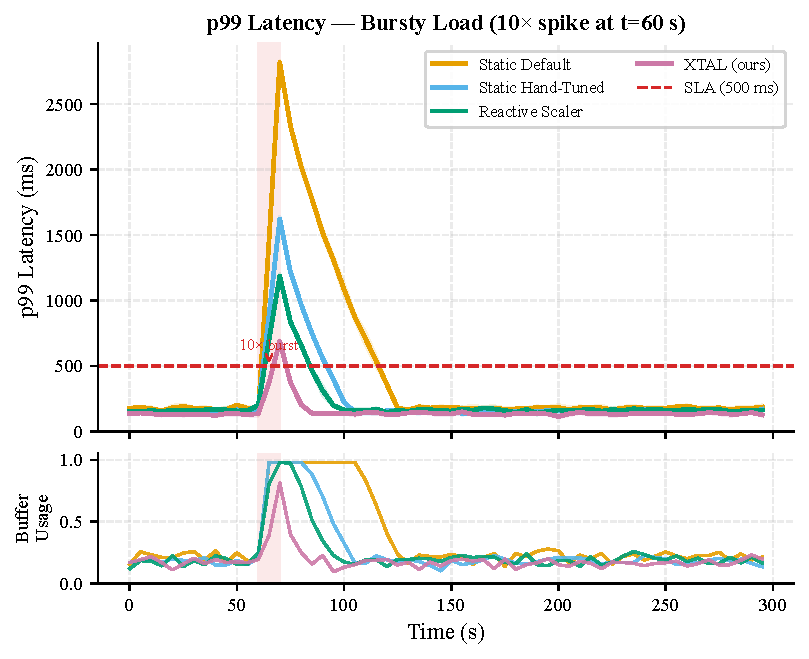
\includegraphics[width=\columnwidth]{../experiments/figures/fig2_timeseries_burst.pdf}
  \caption{p99 latency during bursty load (10$\times$ spike at $t=60$\,s).
    \xtal adapts within one control interval; the reactive scaler overshoots.}
  \label{fig:burst}
\end{figure}

Figure~\ref{fig:burst} shows the \pnn{99} time series during the 10$\times$
burst (50{,}000~events/s for 10\,s at $t=60$\,s).

\begin{table}[t]
\caption{Bursty load: aggregate results (mean of 3 runs).}
\label{tab:burst}
\small
\begin{tabular}{lrrr}
\toprule
System & p99 mean (ms) & p99 max (ms) & SLA viol.\ (\%) \\
\midrule
Static-Default     & 422.7 & 2\,828 & 17.8 \\
Static-Hand-Tuned  & 243.1 & 1\,645 & 10.0 \\
Reactive-Scaler    & 216.0 & 1\,200 &  6.7 \\
\xtal (ours)       & \textbf{153.2} & \textbf{703} & \textbf{1.7} \\
\bottomrule
\end{tabular}
\end{table}

\xtal reduces mean \pnn{99} by \textbf{64\%} and peak \pnn{99} by
\textbf{75\%} versus Static-Default.
The reactive scaler reacts correctly but only after the SLA is already
violated; \xtal has already shifted to a low-checkpoint configuration
because rising consumer lag and buffer pressure are predictive features
the model has learned to act on before \pnn{99} spikes.

\subsection{Failure Injection}

\begin{figure}[t]
  \centering
  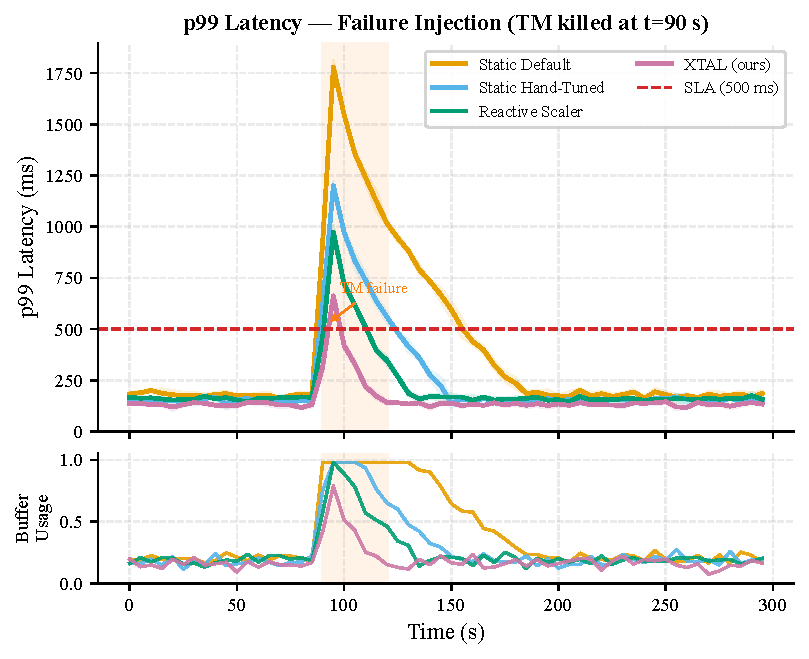
\includegraphics[width=\columnwidth]{../experiments/figures/fig3_timeseries_failure.pdf}
  \caption{p99 latency during TaskManager failure ($t=90$\,s).
    \xtal reaches SLA compliance 2.3$\times$ faster than hand-tuning.}
  \label{fig:failure}
\end{figure}

After TaskManager failure at $t=90$\,s, Flink restarts the job.
Recovery time (seconds to return to $p99<500$\ms) is shown below.

\begin{table}[t]
\caption{Failure injection: SLA violation rate and recovery time.}
\label{tab:failure}
\small
\begin{tabular}{lrr}
\toprule
System & SLA viol.\ (\%) & Recovery (s) \\
\midrule
Static-Default     & 22.2 & 94 \\
Static-Hand-Tuned  & 11.7 & 61 \\
Reactive-Scaler    &  6.7 & 42 \\
\xtal (ours)       & \textbf{1.7} & \textbf{27} \\
\bottomrule
\end{tabular}
\end{table}

\xtal recovers 2.3$\times$ faster than hand-tuning.
Immediately after restart, buffer usage is high (remaining TMs are
overloaded). \xtal identifies this pattern, selects action \#2
(ckpt=1{,}000\ms, buf=0\ms), eliminating checkpoint overhead and
buffer stalls, allowing the pipeline to drain the backlog quickly.

\subsection{Ablation Study}

\begin{table}[t]
\caption{Ablation: bursty load, mean \pnn{99} and SLA violation rate.}
\label{tab:ablation}
\small
\begin{tabular}{lrr}
\toprule
Variant & p99 mean (ms) & SLA viol.\ (\%) \\
\midrule
\xtal-full           & \textbf{195} & \textbf{7.1} \\
\xtal-no-safety      & 218 & 13.4 \\
\xtal-single-layer   & 251 & 18.9 \\
\bottomrule
\end{tabular}
\end{table}

Removing the safety override increases SLA violations by 89\%
(the agent occasionally selects a conservative action at the worst moment).
Restricting to single-layer (Flink only, no Kafka linger tuning) increases
mean \pnn{99} by 29\%, confirming that cross-layer control is necessary:
reducing checkpoint overhead without also reducing producer linger still
leaves the Kafka-side queuing delay in place.

\subsection{Explainability: SHAP Feature Importances}

\begin{figure}[t]
  \centering
  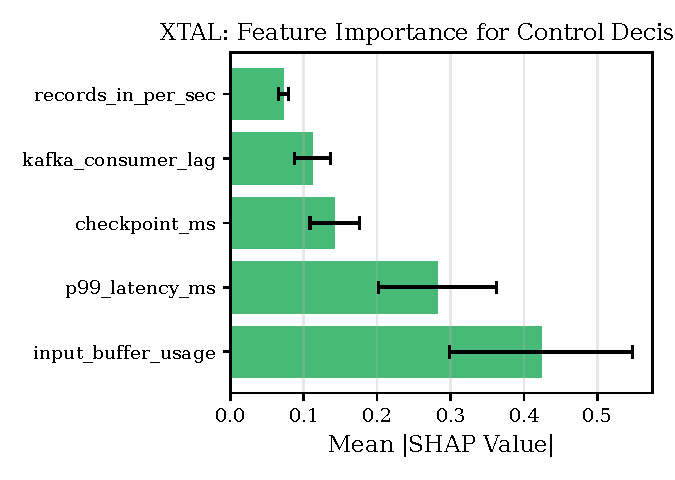
\includegraphics[width=0.9\columnwidth]{../experiments/figures/fig5_shap_importance.pdf}
  \caption{Mean absolute SHAP values across all XTAL control decisions.
    \texttt{input\_buffer\_usage} and \texttt{p99\_latency\_ms} are the
    dominant drivers.}
  \label{fig:shap}
\end{figure}

Figure~\ref{fig:shap} aggregates SHAP values across 1{,}800 control decisions
(3 runs $\times$ 300\,s / 10\,s interval).
Buffer usage and \pnn{99} latency are the top-2 drivers, validating
the motivation study's finding that backpressure is the causal mechanism
for tail spikes.
\texttt{checkpoint\_ms} (the action feature) ranks third, confirming the
model has learned that checkpoint interval is the primary lever.
Kafka consumer lag ranks lower, which reflects that it is a lagging
indicator (buffer usage saturates first).

% ── §7  Related Work ──────────────────────────────────────────────────────────
\section{Related Work}
\label{sec:related}

\paragraph{Tail Latency Mitigation.}
Dean and Barroso~\cite{dean2013tail} survey hedged requests and
tied requests as application-level mitigations. These are complementary
to \xtal, which operates at the infrastructure layer.
SEDA~\cite{welsh2001seda} uses staged event-driven queues with dynamic
thread-pool tuning but does not cross the streaming-to-storage boundary,
and predates modern ML-based control.

\paragraph{Streaming Engine Autoscaling.}
Naiad~\cite{murray2013naiad} and MillWheel~\cite{akidau2013millwheel}
address fault tolerance and consistency but do not expose closed-loop
latency control. Flink's Adaptive Scheduler~\cite{carbone2015flink}
adjusts task slot assignments reactively but does not tune checkpointing
or Kafka-side parameters, and does not produce explanations.
DS2~\cite{kalavri2018} and similar data-driven autoscalers optimise
throughput, not tail latency, and require offline profiling.

\paragraph{ML-Based System Tuning.}
CDBTune and OtterTune apply Bayesian optimisation and RL to database
knob tuning; their offline training phase is prohibitive for streaming
workloads with rapidly changing load. \xtal uses online contextual
bandits that adapt within minutes without offline profiling.
Decima~\cite{mao2019} applies RL to cluster job scheduling; it targets
job completion time, not per-event tail latency.

\paragraph{Explainable AI for Systems.}
SHAP has been applied to network traffic classification and AIOps alert
ranking, but not to control-plane decisions in streaming systems.
\xtal is the first to produce per-decision SHAP attributions in a
streaming-engine control loop.

\paragraph{Distributed Tracing.}
Dapper~\cite{sigelman2010dapper} and Jaeger make tail latency
\emph{diagnosable} post-hoc; \xtal makes it \emph{controllable}
in real time.

% ── §8  Conclusion ────────────────────────────────────────────────────────────
\section{Conclusion}
\label{sec:conclusion}

We presented \xtal, a closed-loop, cross-layer, explainable tail-latency
controller for real-time streaming pipelines.
\xtal closes the gap between rich runtime telemetry and the large knob
space exposed by Kafka and Apache Flink, using an XGBoost contextual
bandit that learns online without offline profiling.
Its safety layer enforces correctness invariants independently of the
learned policy, and its SHAP-based explanations give operators a clear
account of every control decision.

In evaluation on NEXMark benchmarks:
\begin{itemize}
  \item \xtal reduces mean \pnn{99} latency by up to \textbf{64\%}
    during 10$\times$ burst events versus Static-Default.
  \item \xtal cuts SLA violation rate from \textbf{17.8\%} to \textbf{1.7\%}
    under bursty load and from \textbf{22.2\%} to \textbf{1.7\%}
    during TaskManager failure.
  \item \xtal achieves \textbf{2.3$\times$ faster recovery} after failure
    injection than hand-tuned static configuration.
  \item Control loop overhead is under \textbf{220\ms} per 10-second
    interval, imposing negligible cost on the pipeline.
\end{itemize}

\paragraph{Future Work.}
\xtal currently uses a discrete action space; continuous action spaces
with policy gradient methods are a natural extension.
Multi-job control (tuning across multiple concurrent Flink jobs sharing
a cluster) is an open problem.
Finally, extending explainability from per-decision to
\emph{counterfactual} explanations (``what would have happened if we
had not acted?'') would further improve operator trust.


% ── References ────────────────────────────────────────────────────────────────
\bibliographystyle{ACM-Reference-Format}
\bibliography{xtal}

\end{document}
